\section{Klassische Methoden}
Im Folgenden werden nun die bisherigen Ansätze auf dem Gebiet der (raum)zeitlichen Vorhersage vorgestellt. Hierzu wird zuerst die Technik der \textit{Verzögerungskoordinaten} eingeführt, welche die Grundlage der Methoden der \textit{Nächsten-Nachbar}-Vorhersage und der \textit{radialen Basisfunktionen} bildet.
 
\subsection{Verzögerungskoordinanten}
\label{sc:delay_reconstruction}
Die \textit{Verzögerungskoordinaten} (Delay Coordinates) können benutzt werden um Zeitreihen zu analysieren und den Phasenraum des ursprünglichen Systems zu rekonstruieren.
Hierbei wird ein Signal $s(t)$ an diskreten Zeitpunkten betrachtet, sodass sich das diskrete Signal $s_n = s(n\Delta t)$ ergibt. Eine solche Rekonstruktion erzeugt hieraus ein Signal, in welchem die Informationen $\delta$ vorheriger Zeitpunkte mit dem Abstand $\tau$ enthalten sind. Somit wird eine höherdimensionale Zeitreihe $\vec{z}_n \in \mathbf{R}^{\delta}$ durch
\begin{align}
	\vec{z}_n = \left(s_{n-(\delta-1)\tau}, s_{n-(\delta-2)\tau}, \ldots ,s_n \right)
\end{align} 
konstruiert \citep[35\,ff.]{kantz2004nonlinear}. Bei einer ausreichend hohen Wahl der Rekonstruktionsdimension $m$ ist es hiermit möglich den Phasenraum des Attraktors zu rekonstruieren. Für die Wahl der Verzögerungszeit $\tau$ gibt es keine rigorose mathematische Definition oder Beschreibung, sondern es existieren verschiedene Ansätze zur Ermittlung des optimalen Wertes. Ein populärer Ansatz, welcher in dieser Arbeit verwendet wird, besteht darin, $\tau$ durch das Auffinden der ersten Nullstelle der Autokorrelationsfunktion 
\begin{align}
AUC(\tau) = \sum_l^{N-\tau} (s_l-\bar{s})(s_{l+\tau}-\bar{s})
\end{align}   
zu ermitteln. Dies lässt sich dadurch motivieren, dass durch das Hinzunehmen von Signalen der Zeitreihe, die um diesen Wert $\tau$ verschoben sind, am meisten neue Information hinzugefügt wird, da die Selbstähnlichkeit des Signals am geringsten ist \citep[30\,ff.]{kantz2004nonlinear}.
Die so konstruierte höherdimensionale Zeitreihe beinhaltet somit also nicht nur Informationen über den aktuellen Zustand des Systems, sondern auch über die unmittelbare Vergangenheit. Dadurch können diese rekonstruierten Datenpunkte auch genutzt werden, um das Verhalten dynamischer Systeme vorherzusagen. Hierfür werden im Folgenden zwei Methoden eingeführt.
\subsection{Nächster Nachbar Vorhersage}
\label{sc:theory_nn}
Die erste Methode um mittels der zuvor konstruierten höherdimensionalen Zeitreihen Vorhersagen zu treffen ist die \textit{nächste Nachbar}-Vorhersage (im Folgenden als \textsc{NN}-Ansatz abgekürzt). Das allgemeine Ziel \textit{NN}-Vorhersage besteht darin den funktionalen Zusammenhang $F : X \rightarrow Y$ zu finden, welcher Daten der Menge $X \in \mathbb{R}^n$ auf Elemente aus $Y \in \mathbb{R}^m$ eindeutig abbildet. Hierfür wird angenommen, dass die Funktion $F$ lokal stetig ist. Zudem werden hierfür Daten benötigt, anhand derer der Zusammenhang erlernt werden kann. Die Anzahl dieser Trainingsdaten wird im Folgenden mit $N$ bezeichnet.\\
Zu Beginn werden Paare $(\vec{x},\vec{y}) \in X \times Y$ aus einem \textit{Trainingsdatensatz} gebildet und eine Suchstruktur über die $x$-Werte gebildet. Nun kann diese Struktur genutzt werden, um für ein gegebenes $\vec{x}$ den wahrscheinlichsten Wert $\vec{y}$ zu suchen. Hierfür werden, unter der Annahme der lokalen Stetigkeit, die Datenpunkte $\vec{x}_1, ..., \vec{x}_k$ aus der zuvor angelegten Suchstruktur ausgewählt, welche den geringsten Abstand $d(\vec{x}, \vec{x_i})$ zu $\vec{x}$ besitzen.\\
Diesen $k$ Datenpunkten ist jeweils ein eindeutiger Wert $\vec{y}_i$ zuvor zugeordnet werden. Damit kann nun eine Approximation für den zu $\vec{x}$ gehörigen Wert $\vec{y}$ erstellt werden, indem beispielsweise ein gewichteter Mittelwert der $\vec{y}_i$ genutzt wird. Hierzu kann jedem der $k$ nächsten Nachbarn $(\vec{x}_i, \vec{y}_i)$ ein Gewicht $w_i(\vec{x})$ nach
\begin{align*}
w_i(\vec{x}) = \frac{v_i}{\sum_j v_j}, \text{ mit } v_i = \frac{1}{||\vec{x}_i-\vec{x}||} 
\end{align*}
zugeordnet werden. Diese Definition erfüllt $\sum_i w_i = 1$ und ordnen zudem fernen Nachbarn ein geringeres Gewicht zu. Die dabei auftretende Norm $||\cdot ||$ wird im Folgenden als euklidisch angenommen, sofern keine weiteren Angaben existieren. Somit ergibt sich für die gewichtete Vorhersage
\begin{align}
F(\vec{x}) = \vec{y} = \sum^k_i \vec{y}_i \left( \sum_j \frac{||\vec{x}_i-\vec{x}||}{||\vec{x}_j-\vec{x}||} \right) ^{-1}.
\end{align}

Der Schlüssel in der Bewältigung einer solchen Aufgabe liegt hauptsächlich in der Art und Weise, wie die $k$ nächsten Nachbarn gesucht werden. Hierbei wird im Folgenden ein naiver Ansatz ebenso wie der Algorithmus \textsc{k-d-tree} betrachtet. Bei dem naiven Ansatz (\textit{brute force}) werden die nächsten Nachbarn aus dem unsortierten Trainingsdatensatz durch pures Ausprobieren aller möglichen Punkte ermittelt.

\subsubsection{k-d-tree}
Ein \textsc{k-d-tree} ist eine Spezialform eines Binärbaumes, und eine oftmals genutzte Methode um Suchvorgänge in Datenstrukturen durchzuführen. Das zugrundeliegende Prinzip eines solchen Baumen ist, dass wenn der Punkt $P_1$ weit entfernt von $P_2$ liegt, aber $P_3$ nahe an $P_2$ liegt, so folgt daraus, dass $P_1$ und $P_3$ weit voneinander entfernt liegen müssen. Durch eine solche Argumentation muss bei einem solchem Suchvorgang die Distanz zweier Punkte seltener berechnet werden, wodurch Rechenzeit eingespart werden kann.\\

\begin{figure}[h]
    \centering
    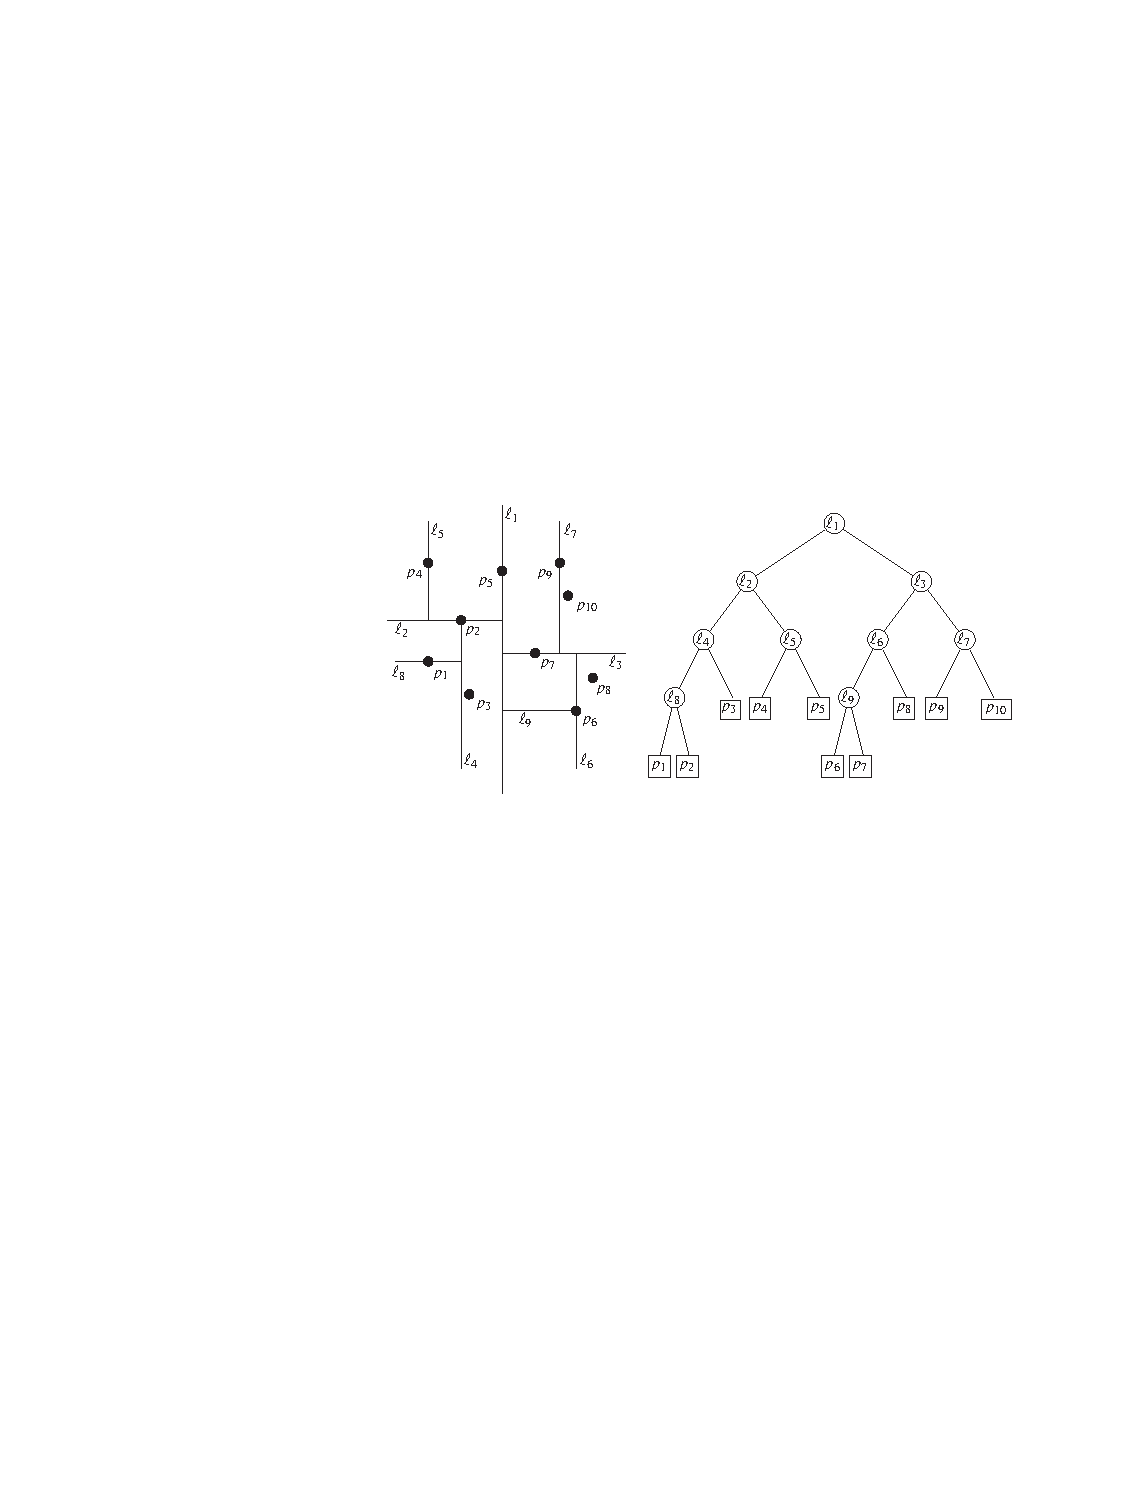
\includegraphics[width = 0.9 \textwidth]{figures/illustrations/kdtree.pdf}
    \caption{Exemplarische Darstellung eines \textsc{k-d-trees} für $d=2$ Dimensionen. In der linkten Hälfte ist die graphische Interpretation der Aufteilung und in der rechten der Aufbau des entstehenden Baumes zu finden \cite{de2000computational}. Der in der $i$-ten Iteration bestimmte Median ist als $l_i$ eingetragen. An jeder Astgabelung werden die Elemente falls sie kleiner als der Median $l_i$ sind in den linken und ansonsten in den rechten Zweig einsortiert.}
    \label{fig:kdtree}
\end{figure}

\improvement{Add search path example to the graph?}

Der Suchvorgang besteht aus zwei Phasen. Zuerst wird die Aufbauphase des Baumes durchgeführt, bei der die Trainingsdaten einsortiert und damit ein Suchindex erzeugt wird. Anschließend folgt die Suchphase, bei der der zuvor erstellte Suchindex nach dem nächsten Nachbarn durchsucht wird.\\

In der Aufbauphase wird zuerst eine Dimensionen ausgewählt und der Median $l_i$ der Daten in dieser Dimension bestimmt. Dieser Wert bildet eine Trennlinie, anhand derer die Punkte in zwei Mengen unterteilt werden, die entweder nur größere oder nur kleinere Elemente bezogen auf jene Dimension beinhalten. Die beiden Mengen bilden die ersten Äste des Baumes. Nun wird dieser Schritt rekursiv auf alle Äste angewendet, und die hierbei zum Vergleich genutzte Dimension iteriert \cite{de2000computational}. Dieses Verfahren wird so lange wiederholt, bis eine bestimmte maximale Anzahl $N_{max}$ an Knotenpunkten pro Ast erreicht wird. Ab dieser unteren Grenze wird das Erstellen des Binärbaumes beendet. Ab dieser Grenze benötigt der Zugriff auf die verschiedenen Elemente und das Aufteilen in neue Äste mehr Zeit, als das Berechnen der Abstände zwischen den verbleibenden $N_{max}$ Knoten und dem Suchpunkt. Eine beispielhafte Darstellung des Verfahrens ist in Abbildung \ref{fig:kdtree} zu finden.

Die Suchphase wird nun wieder rekursiv durchgeführt. Hierbei werden wieder iterierend die verschiedenen Dimensionen verglichen, und sich somit immer weiter im Suchbaum nach unten ein Weg gebahnt \cite{de2000computational}. In der untersten Ebene, also wenn nur noch eine Suche zwischen maximal $N_{max}$ Elemente durchgeführt werden muss, wird nun die \textit{brute force}-Suche genutzt. In dieser Arbeit ist für alle Anwendungen diese Schwelle auf $N_{max} = 40$ gesetzt worden \citep{scikitlearnneighbours}.\\

Diese Methode zeichnet sich durch eine Laufzeit aus, welche sich für einen einzelnen Suchvorgang wie $\mathcal{O}(\log(N))$ verhält \cite{bentley1975multidimensional}. Wird die Vorhersage für $m$ Datenpunkte durchgeführt ergibt sich die Laufzeit zu $\mathcal{O}(m\log(N))$. Dies ist geringer, als die Laufzeit eines naiven Suchvorgangs, welche sich wie $\mathcal{O}(mN)$ verhält. Zusätzlich muss bei der Verwendung des \textsc{k-d-tree}s allerdings auch noch die Baumstruktur aufgebaut werden. Hierfür besteht eine ungefähre Laufzeit $\mathcal{O}(N \log(N))$. Zusätzlich besitzt die Laufzeit des \textsc{k-d-tree}s auch eine Abhängigkeit von der Dimensionalität $d$. Es hat sich gezeigt, dass wenn $d$ hinreichend groß ist, die Vorteile geringer werden, und für hohe Dimensionalitäten ($\approx d > 20)$ die Suche ineffizient abläuft \citep{scikitlearnneighbours}.\\


\subsection{Radiale Basisfunktionen}
Eine weitere Methode um einen funktionalen Zusammenhang $F : X \rightarrow Y$ zu finden, welcher Daten der Menge $X \in \mathbb{R}^n$ auf Elemente aus $Y \in \mathbb{R}^m$ eindeutig abbildet, bieten die \textit{radialen Basisfunktionen} (im Folgenden als \textsc{RBF} abgekürzt) an. Auch dafür werden Daten benötigt, anhand derer der Zusammenhang erlernt werden kann. Diese Trainingsdaten sollen im Folgenden aus $N$ Datenpunkten bestehen.\\

Bei diesem Ansatz wird die gesuchte Funktion $F$ als Linearkombination aus vielen radialen Funktionen approximiert. Dafür werden $l$ Elemente $\{\vec{x}_i\}, i=1,...,l$ aus den Trainingsdaten ausgewählt und diese als so genannte \textit{Zentren} $\{\vec{z}_i\}$ genutzt. Hiermit lassen sich die Funktionen als $\phi_i(\vec{x}) = \phi(||\vec{x}-\vec{z}_i||), i=1,\ldots ,l$ darstellen \citep{lowe2multi}. Eine mögliche Wahl der Basisfunktionen sind zum Beispiel Gaußfunktionen
\begin{align*}
\phi_i(\vec{x}) = \exp \left( - \frac{||\vec{x}-\vec{z}_i||}{\sigma_{RBF, i}^2} \right),
\end{align*}
wobei $\sigma_{RBF, i}$ für die Breite der $i$-ten Gaußfunktion steht.
Die Linearkombination führt zu dem Ansatz 
\begin{align}
\label{eq:rbf_lincomb}
\vec{y} = F(\vec{x}) = \sum^l_{i=1} \vec{\omega}_i \phi(||\vec{x} - \vec{z}_i||).
\end{align}
Die $\vec{\omega}_i \in \mathbb{R}^m$ stehen hier für die \textit{Gewichtsvektoren} der einzelnen Basisfunktionen $\phi_i$ im Rahmen der Linearkombination.\\

Das Ziel besteht jetzt darin, die Gewichtsvektoren $\vec{\omega_i}$ approximativ zu bestimmen. Dafür werden zunächst drei Matrizen definiert, durch die das Problem ausgedrückt werden kann.\\
Die Matrix $\mathbf{Y} \in \mathbb{R}^{N \times m}$ repräsentiert die Funktionswerte der Abbildung und beinhaltet als Zeilen die $N$ verschiedenen Funktionswerte $\vec{y}_i$ der Trainingsdaten
\begin{align}
\mathbf{Y} \defeq
\begin{pmatrix}
y_{11} & \ldots  & y_{1m} \\
\vdots & & \vdots \\
y_{N1} & \ldots  & y_{Nm} \\
\end{pmatrix}.
\end{align}
Die Matrix $\mathbf{\Omega} \in \mathbb{R}^{l \times m}$ beinhaltet dagegen als Zeilen die Gewichtsvektoren
\begin{align}
\mathbf{\Omega} \defeq
\begin{pmatrix}
\omega_{11} & \ldots  & \omega_{1m} \\
\vdots & & \vdots \\
\omega_{l1} & \ldots  & \omega_{lm} \\
\end{pmatrix}.
\end{align}
Die dritte Matrix $\mathbf{A} \in \mathbb{R}^{N \times m}$ repräsentiert Anwendungen der radialen Basisfunktionen auf die Trainingsdaten 
\begin{align}
\mathbf{A} \defeq
\begin{pmatrix}
A_{11} & \ldots  & A_{1m} \\
\vdots & & \vdots \\
A_{N1} & \ldots  & A_{Nm} \\
\end{pmatrix},
\end{align}
wobei die einzelnen Elemente als $A_{ij} \defeq \phi(|| \vec{x}_i - \vec{y}_j ||)$ definiert sind.\\
Das Problem lässt sich somit durch
\begin{align}
\mathbf{Y} = \mathbf{A} \cdot \mathbf{\Omega}
\end{align}
ausdrücken \citep{lowe2multi}. Da die Matrizen $\mathbf{Y}$ und $\mathbf{A}$ konstruiert sind, besteht die Aufgabe lediglich darin die Matrix $\mathbf{\Omega}$ der Gewichte zu ermitteln. Der naheliegende Ansatz, das direkte Ermitteln der Inversen $\mathbf{A}^{-1}$ stellt sich dafür aus ungeeignet heraus, da das Problem meistens überkonditioniert ist und die Matrix nicht quadratisch ist, wodurch keine Inverse gefunden werden kann. Stattdessen ist es geschickter, das Problem als eine lineare Optimierungsaufgabe zu betrachten, bei der der Fehler $||\mathbf{A} \vec{\omega_i} - \vec{y}_i||^2$ minimiert werden soll.\\
Durch die Verwendung der \textit{Moore-Penrose Pseudoinversen} $\mathbf{A}'$ wird zugleich gewährleistet, dass die Lösung ausgewählt wird, die zudem auch die kleinsten Gewichte besitzt. Dies hilft den Effekt des \textit{Overfittings} zu verringern \cite{lowe2multi}. Das \textit{Overfitting} beschreibt den Effekt, dass das Vorhersage-Modell zu stark auf die Trainingsdaten angepasst ist, und das Verhalten nicht stark genug generalisiert. Dies ist an einem (deutlich) höheren Test- als Trainingsfehler zu erkennen.\\

Mit diesem Ansatz ergibt sich die Lösung zu
\begin{align}
\mathbf{\Omega} = \mathbf{A}' \cdot \mathbf{Y}.
\end{align}

Um nun Funktionswerte vorherzusagen, wird der oben eingeführte Zusammenhang \ref{eq:rbf_lincomb} zwischen den zuvor ermittelten Gewichten und der Zielvariable $\vec{y}$ genutzt.